\documentclass[10pt]{beamer} %Beamer

\usepackage{palatino} %font type
\usepackage{caption}
\usepackage{hyperref}
\usepackage[T1]{fontenc}
\usepackage{listings}
\usepackage{csquotes}


\usepackage{appendixnumberbeamer} %enumerate each slide without counting the appendix

%These next packages are the useful for Physics in general, you can add the extras here.
\usepackage{amsmath,amssymb}
\usepackage{slashed}
\usepackage{dirtree}
\usepackage{relsize}
\usepackage{multirow}
\usepackage{caption}
\usepackage{subcaption}
\usepackage{multicol}
\usepackage{booktabs}
\usepackage[scale=2]{ccicons}
\usepackage{pgfplots}
\usepgfplotslibrary{dateplot}
\usepackage{geometry}
\usepackage{xspace}
\usepackage{color}

\lstloadlanguages{C,C++,csh,Java}
\usefonttheme{metropolis} %Type of slides
\usefonttheme[onlymath]{serif} %font type Mathematical expressions
\usetheme[progressbar=frametitle,titleformat frame=smallcaps,numbering=counter]{metropolis} %This adds a bar at the beginning of each section.
\useoutertheme[subsection=false]{miniframes} %Circles in the top of each frame, showing the slide of each section you are at

\definecolor{red}{rgb}{0.6,0,0}
\definecolor{blue}{rgb}{0,0,0.6}
\definecolor{green}{rgb}{0,0.8,0}
\definecolor{cyan}{rgb}{0.0,0.6,0.6}

\lstset{
language=csh,
basicstyle=\footnotesize\ttfamily,
numbers=left,
numberstyle=\tiny,
numbersep=5pt,
tabsize=2,
extendedchars=true,
breaklines=true,
frame=b,
stringstyle=\color{blue}\ttfamily,
showspaces=false,
showtabs=false,
xleftmargin=17pt,
framexleftmargin=17pt,
framexrightmargin=5pt,
framexbottommargin=4pt,
commentstyle=\color{green},
morecomment=[l]{//}, %use comment-line-style!
morecomment=[s]{/*}{*/}, %for multiline comments
showstringspaces=false,
morekeywords={ abstract, event, new, struct,
as, explicit, null, switch,
base, extern, object, this,
bool, false, operator, throw,
break, finally, out, true,
byte, fixed, override, try,
case, float, params, typeof,
catch, for, private, uint,
char, foreach, protected, ulong,
checked, goto, public, unchecked,
class, if, readonly, unsafe,
const, implicit, ref, ushort,
continue, in, return, using,
decimal, int, sbyte, virtual,
default, interface, sealed, volatile,
delegate, internal, short, void,
do, is, sizeof, while,
double, lock, stackalloc,
else, long, static,
enum, namespace, string},
keywordstyle=\color{cyan},
identifierstyle=\color{red},
backgroundcolor=\color{white},
}
\usepackage{biblatex}
\usepackage{caption}
\DeclareCaptionFont{white}{\color{white}}
\DeclareCaptionFormat{listing}{\colorbox{blue}{\parbox{\textwidth}{\hspace{15pt}#1#2#3}}}
\captionsetup[lstlisting]{format=listing,labelfont=white,textfont=white, singlelinecheck=false, margin=0pt, font={bf,footnotesize}}
\newcommand{\themename}{\textbf{\textsc{bluetemp}\xspace}}%metropolis}}\xspace}

\title{CTFEF }
\subtitle{Building a compiler for metaprogramming languages}
\author[name]{
	Adam Grabski\\
	Ilona Bluemke
}

\institute[uni]{Institute of Computer Science \\
Department of Electronics and Information Technology \\
Warsaw Univeristy of Technology
}
\date{September 18, 2023} %Here you can change the date
\begin{document}
{

\maketitle
}%This is the colour of the first slide. bg= background and fg=foreground
\AtBeginSection{}

\begin{frame}{Agenda}
	\setbeamertemplate{section in toc}[sections numbered] %This is numbering the sections
	\tableofcontents[subsectionstyle=hide/hide/hide] %You can comment this line if you want to show the subsections in the table of contents
\end{frame}

\section{Motivation}


\begin{frame}
	\frametitle{Motivation}

	\begin{itemize}
		\item Metaprogramming - writing programs that analyse or modify themselves\begin{itemize}
			      \item Dynamic - metaprogramming done at run time
			      \item Static - metaprogramming done at compile time
		      \end{itemize}
		\item Makes code more expressive and resilient to change
		\item Boosts productivity
		\item Can improve performance
		\item Mostly present in garbage-collected languages at runtime\begin{itemize}
			      \item C\#
			      \item Java
			      \item Scripting languages such as Javscript or python
		      \end{itemize}
	\end{itemize}

\end{frame}


\begin{frame}
	\frametitle{Static metaprogramming}

	\begin{itemize}
		\item Until recently a niche tool \begin{itemize}
			      \item C style preprocessor macros
			      \item D templates, compile time function execution and string mixins
		      \end{itemize}
		\item Significant developments since 2011\begin{itemize}
			      \item C++ SFINAE template metaprogramming (standardized 2011)
			      \item Rust procedural macros (introduced with the language in 2015)
			      \item C\# source generators (introduced in 2020)
		      \end{itemize}

		\item Significant current interest and more development in the future\begin{itemize}
			      \item Migration of many typical dynamic metaprogramming activities to compile time in C\#
			      \item Introduction of compile time interceptors in C\#12
			      \item Continuous development of generic programming in C++
		      \end{itemize}
	\end{itemize}

\end{frame}

\begin{frame}[fragile]
	\frametitle{Motivating example}
	\begin{lstlisting}
struct person {
	std::string name;
	int yearOfBirth;
	int height;
};
void print(
  std::ostream&s,
  person const& p) {
  s << p.name << '\n'
    << p.yearOfBirth << '\n'
    << p.height << '\n';
}
	\end{lstlisting}

\end{frame}

\begin{frame}
	\frametitle{C-=-1}

	\begin{itemize}
		\item General purpose, compiled research programming language with manual memory management
		\item Built around powerful static metaprogramming features
		\item Arbitrary code can be executed at compile time\begin{itemize}
			\item Inspect the code base and report diagnostics
			\item Access semantic information generated by the compiler
			\item Modify the program before it is translated to machine code
			\item Access the file system and external tools
		\end{itemize}
	\end{itemize}

\end{frame}


\section{CTFEF}

\begin{frame}
    \frametitle{CTFEF compiler architecture}
    \begin{figure}
        
        \begin{center}
            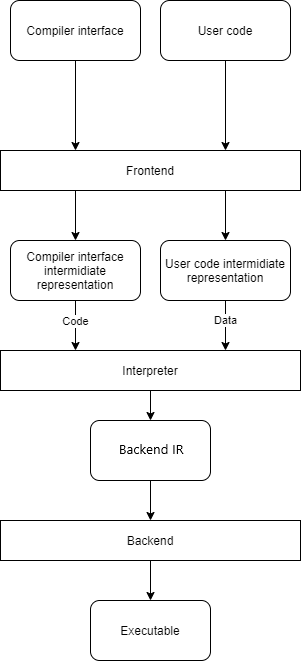
\includegraphics[height=6cm]{pictures/compiler-structure.png}
        \end{center}
    \end{figure}

\end{frame}


\begin{frame}
    \frametitle{Frontend}

    \begin{itemize}
        \item Translates source code into Intermediate Representation\begin{itemize}
            \item Parse
            \item Validate syntax
            \item Inline operators with special syntax (ex: \lstinline|typeof|)
        \end{itemize}
        \item Processes user code and Compiler Interface \begin{itemize}
            \item Compiler Interface translates user code into backend Intermediate Representation
        \end{itemize}
        \item May perform additional processing\begin{itemize}
            \item In C-=-1 it invokes the interpreter to execute metaprogramming code
        \end{itemize}
    \end{itemize}

\end{frame}

\begin{frame}
    \frametitle{Intermediate Representation}

    \begin{itemize}
        \item Complete representation of the user program
        \item Simplified form of the compiled language\begin{itemize}
            \item Resolved function overloads
            \item Advanced constructs lowered to basic ones (foreach loops transformed into while)
        \end{itemize}
        \item Stored using Interpreter data structures in compiler memory\begin{itemize}
            \item Reduces the need for marshalling between interpreted code and the compiler
            \item Introduces significant amount of indirection to all data structures
        \end{itemize}
    \end{itemize}

\end{frame}

\begin{frame}
    \frametitle{Interpreter}

    \begin{itemize}
        \item Operates on Intermediate Representation 
        \item Uses the same data structures for code and data
        \item Allows executing arbitrary code \begin{itemize}
            \item In practice some operations make sens only at runtime
            \item Some operations must be done slightly differently between runtime and compiletime (ex: memory management)
        \end{itemize}
        \item Must expose api for generating backend IR\begin{itemize}
            \item In case of C-=-1 bindings for parts of LLVM library were created
        \end{itemize}
    \end{itemize}

\end{frame}

\begin{frame}
    \frametitle{Backend}

    \begin{itemize}
        \item Module that generates machine code based on IR generated by Compiler Interface
        \item No constraints are placed on this module by CTFEF architecture
        \item In case of C-=-1 compiler, LLVM library was used without any modifications
    \end{itemize}

\end{frame}

\section{C-=-1}

\section{Conclusions}

\begin{frame}
    \frametitle{Conclusions}

    

\end{frame}

\begin{frame}
    \frametitle{Conclusions}

    \begin{itemize}
        \item C-=-1 performance is unsatisfactory\begin{itemize}
            \item ~10 minutes to compile 200 lines of code
        \end{itemize}
        \item Performance of the compiler was not a subject of the research, a lot of improvements are possible\begin{itemize}
            \item Currently only debug build works
            \item Interpreter data structures are inefficient (significant amount of indirection when accessing object members)
        \end{itemize}
        \item Further work is needed
    \end{itemize}

\end{frame}


\end{document}
